\section{Conclusion}

In conclusion, the participant in our tests seemed happy with the program after learning how to use it.  However, looking at the interface implementation from a more professional point of view it is clear that some mistakes has been made.  For one thing, there should not be a 50 second plus learning curve on opening an image file.  This is one of the simplest operations a desktop application can make, and this confusion was entirely avoidable had the designers taken the time to implement the standard main menu, File sub-menu pattern found in so many applications.

Having ignored that convention, the programmers placed a vital user interface element at the far right of the window. It is well known in design, and has be born out by research carried out into eye movement tracking, that a person concentrates their gaze to the top and left of an application, and so by placing the list of annotations on the far right they should have considered that it may be more difficult for the user to spot and consequently re-thought that placement.  

Finally, it is typical in every day computer use that clicking on a UI component will either highlight or select it.  By separating the place where you select an annotation from the place where it is drawn you are disregarding this paradigm, and ultimately this can only lead to confusion on the users part.

Design deficiencies are clearly demonstrated in Figure \ref{fig:ave_rate} when the time to complete a task for the first time is plotted against user rating of how easy the task was.

\begin{figure}[t]
\centering
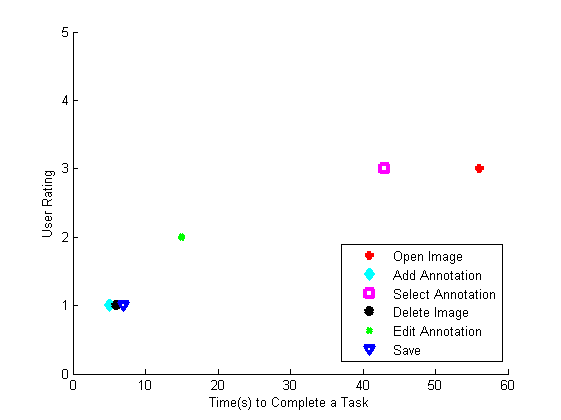
\includegraphics[width=9cm]{average_rating.png}
\caption{time takes for completing a task for the first time plotted against user rating of how easy it was to accomplish the task, lower number indicates task was easier. }
\label{fig:ave_rate}
\end{figure}

Since the application is so simple it gets away with having a bit of a quirky layout, at least as far as our test subject was concerned.  However, in terms of following HCI principles, this application breaches a few too many and so we feel it would be better to redo the design in a more conventional manner so that users may be less confused while using it.  